\section{Legge di Gauss}

\subsection{Flusso del campo elettrico}
Il flusso $\Phi$ di un campo elettrico uniforme $\vec{E}$ attraverso una superficie piana $\Delta \vec{S}$ è:
\begin{equation}
    \Phi_E = \vec{E}\cdot \Delta\vec{S} = E\Delta S \cos\theta
\end{equation}
\begin{figure}[H]
    \centering
    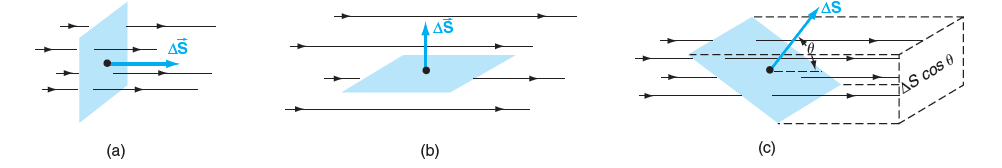
\includegraphics[width=1\linewidth]{imgs/3 - flusso gauss.png}
    \label{fig:flusso}
    \caption{Flusso rispetto al piano}
\end{figure}

\subsection{Flusso attraverso superfici non piane}
Si utilizza l'integrale.
\begin{equation}
    \Phi_E = \lim_{\Delta S_i \to 0} \sum_i{\vec{E_i}\cdot\Delta\vec{S_i}} = \iint{\vec{E}\cdot d\vec{S}} = \iint{E \cos\theta dS}
\end{equation}

Nella maggior parte dei casi si parlerà di integrali di superfici per superficie chiuse
e si indicano con il simbolo:
\begin{equation*}
    \Phi_E = \oiint{\vec{E}\cdot d\vec{S}}
\end{equation*}

\subsection{Legge di gauss}
Il flusso del campo elettrico attraverso una superficie chiusa arbitraria è pari
alla somma algebrica delle cariche contenute all'interno del volume delimitato
dalla superficie divisa per la costante dielettrica del vuoto.

\begin{equation}
    \Phi_E = \frac{Q_{int}}{\epsilon_0}
\end{equation}

\subsection{Superficie gaussiana}
La superficie chiusa attraverso la quale si calcola il flusso del campo elettrico
è solitamente una superficie geometrica immaginaria detta \textbf{superficie gaussina}.

\subsubsection{Esempio}
\begin{figure}[H]
    \centering
    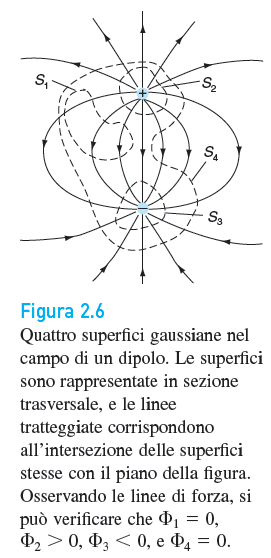
\includegraphics[width=0.25\linewidth]{imgs/4 - superficie gaussiana.png}
    \label{fig:esempio_sup_gaussiana}
    \caption{Esempio superficie gaussiana}
\end{figure}

\subsection{Campo prodotto da carica puntiforme}
\begin{figure}[H]
    \centering
    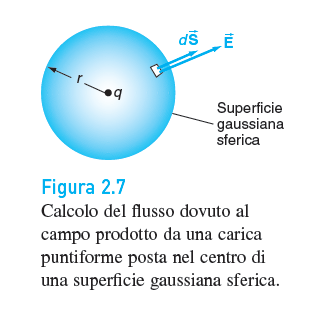
\includegraphics[width=0.25\linewidth]{imgs/5 - calcolo flusso sfera.png}
    \label{fig:esercizio_gauss_sfera}
    \caption{Campo carica puntiforme}
\end{figure}
\begin{equation}
    \Phi_E = \oiint{\vec{E}\cdot d\vec{S}} = E_r(4\pi r^2)
\end{equation}
N.B. $4\pi r^2$ è la superficie della sfera.

Se consideriamo che la carica nella sfera guassiana sia $Q_{int} = q$, 
\begin{equation*}
    \Phi_E = E_r(4\pi r^2) = \frac{q}{4\pi\epsilon_0 r^2}
\end{equation*}
Che è la stessa espressione ottenuta con Coulomb!

\subsection{legge di Coulomb $\Rightarrow$ Legge di Gauss}
\begin{figure}[H]
    \centering
    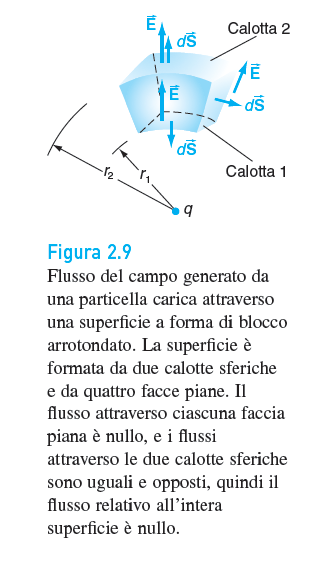
\includegraphics[width=0.25\linewidth]{imgs/6 - flusso esterno.png}
    \label{fig:carica_esterna}
    \caption{Esempio con carica esterna alla superficie}
\end{figure}

\subsubsection{Carica esterna, superficie arbitraria chiusa}
Per una qualunque superficie chiusa arbitraria ed una carica $q$ ESTERNA, il flusso vale:
\begin{equation*}
    \Phi_E = 0
\end{equation*}

\subsubsection{Carica interna, superficie arbitraria chiusa}
\begin{figure}[H]
    \centering
    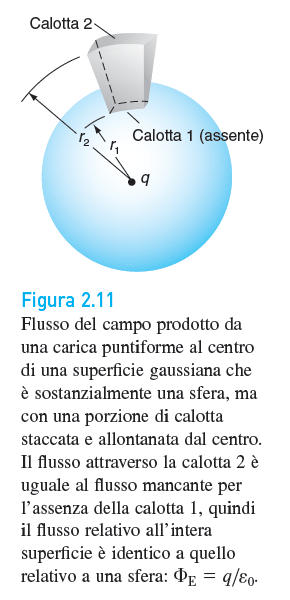
\includegraphics[width=0.25\linewidth]{imgs/7 - figura arbitraria.png}
    \label{fig:carica_interna}
    \caption{Esempio con carica interna alla superficie}
\end{figure}
Per le figure con una carica interna vale:
\begin{equation}
    \Phi_E = \frac{q}{\epsilon_0}
\end{equation}

\subsubsection{Carica sia interna che esterna con superficie chiusa}
\begin{figure}[H]
    \centering
    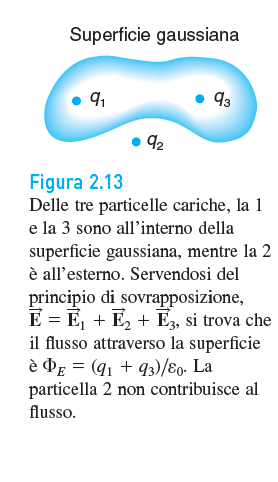
\includegraphics[width=0.25\linewidth]{imgs/8 - cariche esterne ed interne.png}
    \label{fig:carica_sia_interna_che_esterna}
    \caption{Esempio con carica esterna ed interna alla superficie}
\end{figure}

\begin{equation*}
    \Phi_E = \oiint{\vec{E}\cdot d\vec{S}} = \sum_i{\oiint{\vec{E_i}\cdot d\vec{S}}}
\end{equation*}
\begin{equation*}
    \Phi_E = \frac{Q_1}{\epsilon_0} + 0 + \frac{Q_3}{\epsilon_0}
\end{equation*}

\subsection{Legge di Coulomb Vs Legge di Gauss}
La legge di Gauss può essere dedotta da:
\begin{itemize}
    \item legge di Coulomb
    \item principio di sovrapposizione
\end{itemize}
Legge fi Coulomb può essere dedotta da:
\begin{itemize}
    \item legge fi gauss
    \item considerazioni di simmetria
\end{itemize}


\subsection{Carica con simmetria sferica}
Il campo all'esterno di una distribuzione di carica a simmetria sferica è diretto
radialmente e la sua intensità è la stessa che si avrebbe se la carica totale
fosse "concentrata" in una carica puntiforme posta al centro della
distribuzione
\begin{equation*}
    \vec{E} = \frac{q}{4\pi\epsilon_0 r^2}
\end{equation*}

\subsection{Proprietà elettrostiche dei conduttori}
\begin{itemize}
    \item Campo al'interno di un conduttore è nullo
    \item L'eccesso di carica si posiziona sulla superficie
\end{itemize}

\subsection{Campo nelle vicinanze di un conduttore}
Il campo creato dal conduttore è perpendicolare alla superficie.
In prossimità del conduttore, dove la carica di superficie $\sigma>0$, 
$E_n > 0$ avendo una intensità:
\begin{equation}
    E_n = \frac{\sigma}{\epsilon_0}
\end{equation}